\chapter{CN-Wheat: Additional Information} \label{app:cnwheat}

\section{Simulation Details} \label{app:cnwheat-simulation}

We used the post-vegetative simulations used for the ``NEMA'' experiment from \citet{barillot_cn-wheat_2016-1}\footnote{All simulations are available at \url{https://github.com/openalea-incubator/WheatFspm}}. 
We used the simulations for the H0, H3 and H15 fertilization regimes.
The simulations were run as-is for their entire fifty-day duration.


\section{Reservoir Composition} \label{app:cnwheat-reservoir}

In CN-Wheat, photosynthesis occurs in more than just the leaf elements.
Because the structural model is already small at just fifteen elements, we allowed all shoot elements to be part of the reservoir.
This left ten elements that track eco-physiological processes of interest (namely surface temperature $T_s$, transpiration rate $E$, stomatal conductance $g_s$, and net photosynthesis rate $A_n$).
However, we still selected a random sample of seven elements so that the readout model does not have total observability over the internal state of the plant model.


\section{Regression Dataset} \label{app:cnwheat-dataset}

We noticed in initial experiments that the reservoir dynamics have a sudden change at a specific time step in each simulation configuration (see Figure \ref{fig:cnwheat-regime-change}).
The time step is different for each of the fertilization regimes.
Because this regime change likely violates the assumption of a pseudo-static reservoir, we trimmed the output data to only include data from before the regime change.
After trimming, 29, 35, and 37 days of data from the H0, H3 and H15 simulations remain.

Because the same plant is used in all three scenarios, we combined the data into a single dataset; this gives us three different samples per time step.
Model scores trained on the combined dataset were comparable to or slightly lower than models trained using data from a single scenario.
But combining the datasets resulted in a lower variance in scores.
Figure \ref{fig:cnwheat-grouping} illustrates how the simulation data was grouped for train, validation and test splitting.

% TODO: Figure of regime change
% TODO: Figure of dataset grouping

\section{Cross-Validation Strategy} \label{app:cnwheat-validation}

We used the leave-one-group-out strategy from Section \ref{methods:validation} for finetuning the regularization parameter.

\section{Setup Impulse Experiment} \label{app:cnwheat-impulse}

The H3 simulation was used for all impulse experiments.
We applied the stimulus on day 19 of the meteorological inputs from Figure \ref{fig:cnwheat-meteo}. 
Each simulation ran its entire fifty-day course.
The impulse was applied to incident photosynthetically active radiation (\acrshort{par}).
We used amplitudes of 0 and 4000 \unit{\micro\mole\per\square\metre\per\second}. 
The latter corresponds to approximately twice the maximal naturally occurring signal strength. 

% \begin{figure}
%     \centering
%     \begin{subfigure}[b]{0.485\linewidth}
%         \centering
%         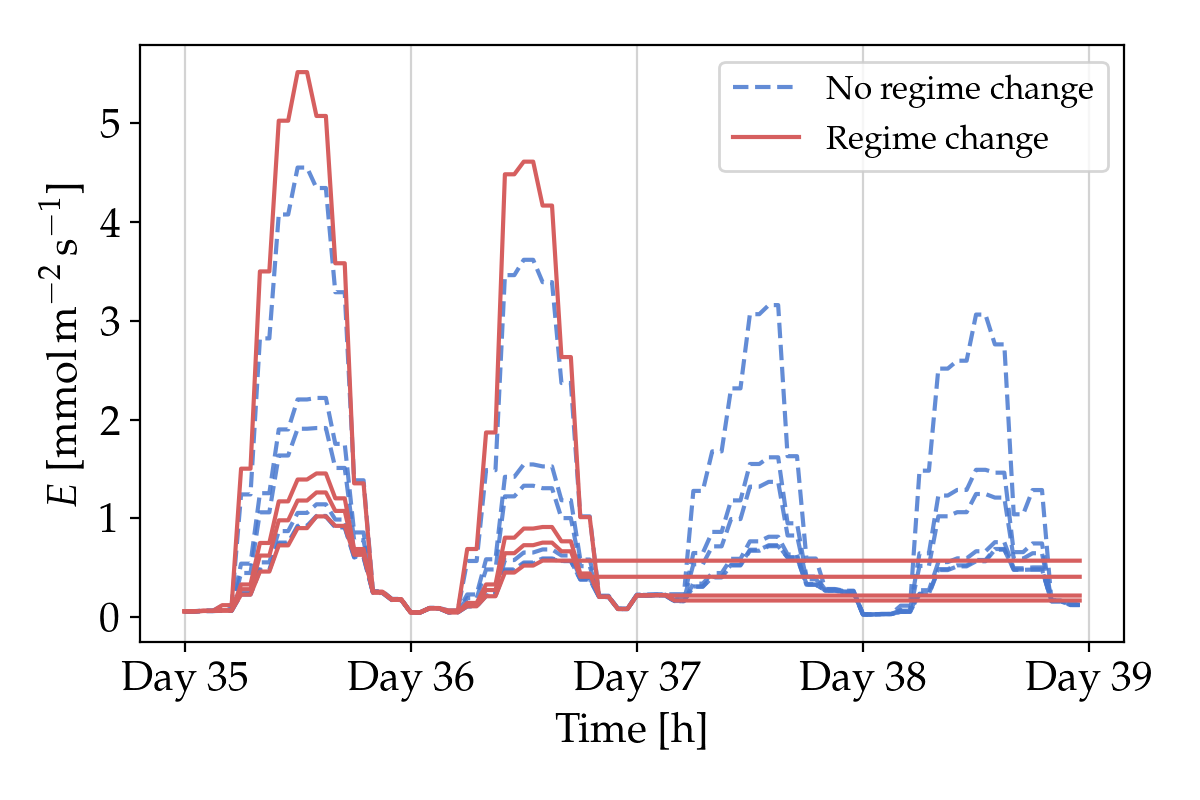
\includegraphics[width=\linewidth,height=\linewidth,keepaspectratio]{img/cn_regime_change.png}
%         \caption{HydroShoot}
%         \label{fig:hydroshoot-archi}
%     \end{subfigure}
%     \hfill
%     \begin{subfigure}[b]{0.485\linewidth}
%         \centering
%         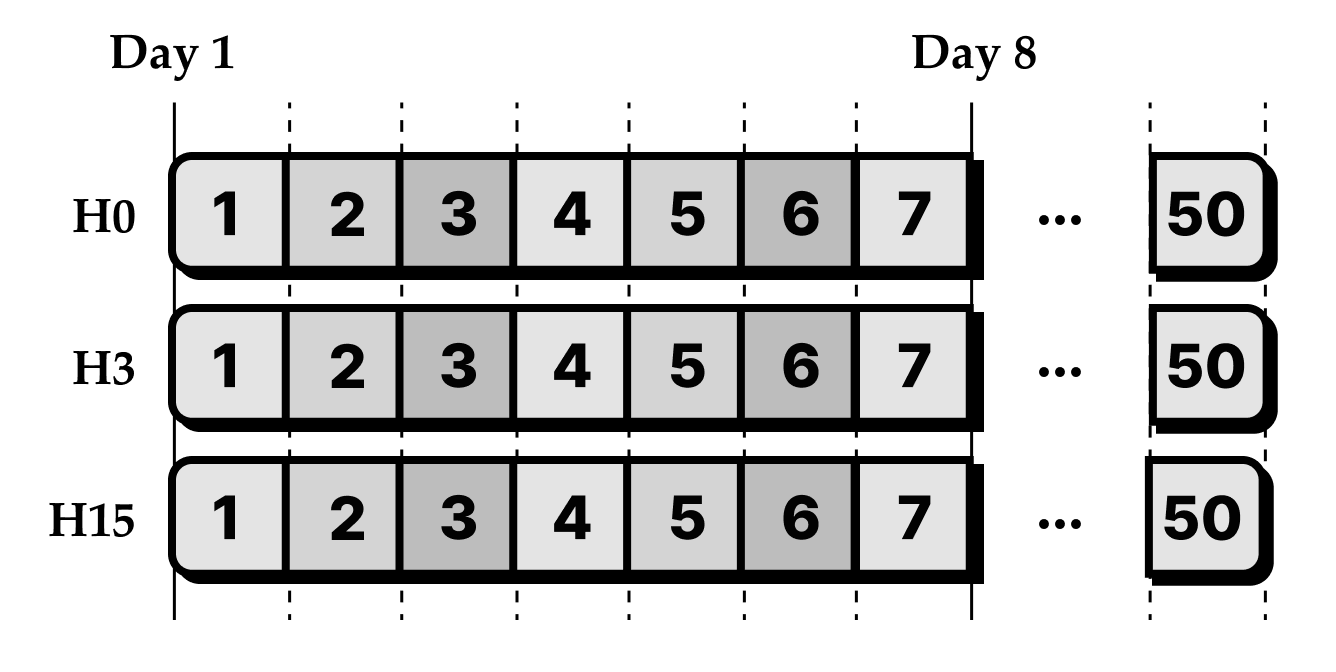
\includegraphics[width=\linewidth,height=0.85\linewidth,keepaspectratio]{img/cnw-grouping.png}
%         \caption{CN-Wheat}
%         \label{fig:cnwheat-archi}
%     \end{subfigure}
%     \caption{
%             FSPMs selected for use in experiments in this work. 
%             (\subref{fig:hydroshoot-archi}) A grapevine specimen from HydroShoot with the canopy trained in the ``Geneva Double Curtain'' configuration.  This figure is reused from \citet{albasha_hydroshoot_2019} under the CC BY 4.0 license.
%             (\subref{fig:cnwheat-archi}) The architecture of the CN-Wheat model. This figure is reused from \citet{barillot_cn-wheat_2016} with permission from the publisher (Copyright 2016 Oxford University Press).
%     }
%     \label{fig:appendix_cnwheat_figures}
% \end{figure}

\begin{figure}[]
	\centering
    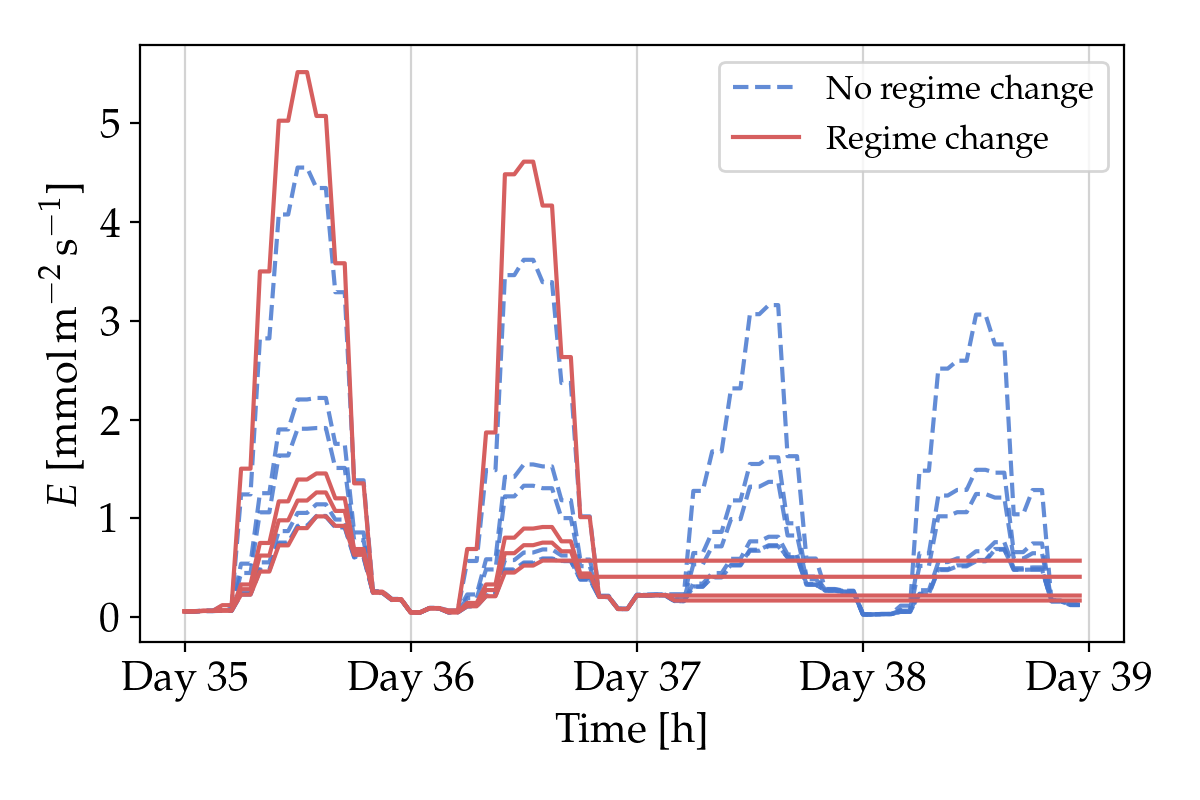
\includegraphics[width=10cm]{img/cn_regime_change.png}
	\caption[Some structural elements of CN-Wheat stop functioning after a specific amount of days.]{Some structural elements of CN-Wheat stop functioning after a specific amount of days. Depicted on the figure is the transpiration rate of each shoot element in the H3 simulation. The red elements change their behavior after day 37.}
	\label{fig:cnwheat-regime-change}
\end{figure}


\begin{figure}[]
	\centering
    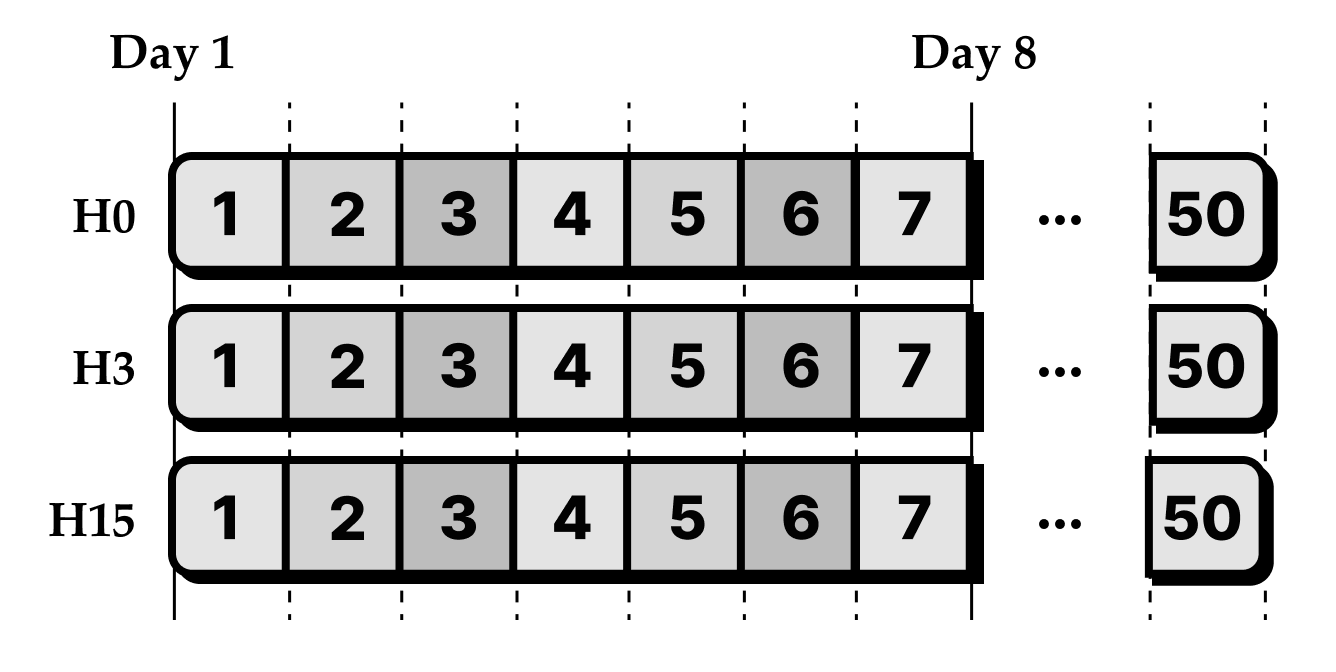
\includegraphics[width=10cm]{img/cnw-grouping.png}
	
	\caption[Data grouping method used to combine data from three simulations of CN-Wheat.]{Data grouping method used to combine data from three simulations of CN-Wheat. Data with the same group number must stay together in a train, validation, or test set.}
	\label{fig:cnwheat-grouping}
\end{figure}

% - Here we always used the H3 variant of the available simulations.
% - Impulse was applied on days X, Y, Z.
% - Impulse was never applied more than once per simulation run; avoided in case the impulse had a lasting effect on the reservoir.
% - We allowed the simulation to run its entire original course.
% - Impulse was applied to I_PAR, with value of 0, and 4000 mol/m2s (+-2x max amplitude in natural signal.)
